\documentclass[journal]{style/vgtc} 			          % final (journal style)
%\documentclass[review,journal]{style/vgtc}         % review (journal style)
%\documentclass[widereview]{style/vgtc}             % wide-spaced review
%\documentclass[preprint,journal]{style/vgtc}       % preprint (journal style)
%\documentclass[electronic,journal]{style/vgtc}     % electronic version, journal

%% Uncomment one of the lines above depending on where your paper is
%% in the conference process. ``review'' and ``widereview'' are for review
%% submission, ``preprint'' is for pre-publication, and the final version
%% doesn't use a specific qualifier. Further, ``electronic'' includes
%% hyperreferences for more convenient online viewing.

%% Please use one of the ``review'' options in combination with the
%% assigned online id (see below) ONLY if your paper uses a double blind
%% review process. Some conferences, like IEEE Vis and InfoVis, have NOT
%% in the past.

%% Please note that the use of figures other than the optional teaser is not permitted on the first page
%% of the journal version.  Figures should begin on the second page and be
%% in CMYK or Grey scale format, otherwise, colour shifting may occur
%% during the printing process.  Papers submitted with figures other than the optional teaser on the
%% first page will be refused.

%% These three lines bring in essential packages: ``mathptmx'' for Type 1
%% typefaces, ``graphicx'' for inclusion of EPS figures. and ``times''
%% for proper handling of the times font family.

\usepackage{mathptmx}
\usepackage{graphicx}
\usepackage{times}

%% We encourage the use of mathptmx for consistent usage of times font
%% throughout the proceedings. However, if you encounter conflicts
%% with other math-related packages, you may want to disable it.

%% This turns references into clickable hyperlinks.
\usepackage[bookmarks,backref=true,linkcolor=black]{hyperref} %,colorlinks
\hypersetup{
  pdfauthor = {},
  pdftitle = {},
  pdfsubject = {},
  pdfkeywords = {},
  colorlinks=true,
  linkcolor= black,
  citecolor= black,
  pageanchor=true,
  urlcolor = black,
  plainpages = false,
  linktocpage
}

%% If you are submitting a paper to a conference for review with a double
%% blind reviewing process, please replace the value ``0'' below with your
%% OnlineID. Otherwise, you may safely leave it at ``0''.
\onlineid{0}

%% declare the category of your paper, only shown in review mode
\vgtccategory{Research}

%% allow for this line if you want the electronic option to work properly
\vgtcinsertpkg

%% In preprint mode you may define your own headline.
%\preprinttext{To appear in an IEEE VGTC sponsored conference.}

%% Paper title.

\title{Interactive Visual Analysis of Image-Centric Cohort Study Data}

%% This is how authors are specified in the journal style

%% indicate IEEE Member or Student Member in form indicated below
\author{TBA}
\authorfooter{
%% insert punctuation at end of each item
% \item
%  Otto-v.-Guericke-University Magdeburg
}

%other entries to be set up for journal
\shortauthortitle{Klemm \MakeLowercase{\textit{et al.}}: Interactive Visual Analytics of Image-Centric Cohort Study Data}
%\shortauthortitle{Firstauthor \MakeLowercase{\textit{et al.}}: Paper Title}

%% Abstract section.
\abstract{Epidemiological population studies impose information about a set of subjects (a \emph{cohort}) to characterize disease specific risk factors.
%
Cohort studies comprise heterogenous variables (\emph{features}) describing the medical condition as well as demographic and lifestyle factors.
%
Using well established statistical methods the data is hypothesis driven analyzed to find statistically significant variable correlations (\emph{interactions}).
%
Modern cohort studies also incorporate medical image data.
%
Analyzing these data requires image segmentation, extraction of key figures and shape based subject grouping.
\\\\
We propose a Interactive Visual Analysis approach that enables epidemiologists to examine both image-based as well as sociodemographic and medical attribute data.
%
It allows for both hypothesis validation approaches as well as hypothesis generation by incorporating data mining methods.
%
Adaptive linked information visualization views and 3d-shape renderings are combined with epidemiological techniques.
%
Similarity measures between data variables are used to compute interesting changes in variable interactions for the current variable selection.
%
Shape based grouping of subjects is facilitated using clustering techniques which operate on surface meshes extracted from the image segmentation.
} % end of abstract


%% Keywords that describe your work. Will show as 'Index Terms' in journal
%% please capitalize first letter and insert punctuation after last keyword
\keywords{Interactive Visual Analytics, Epidemiology}

%% ACM Computing Classification System (CCS). 
%% See <http://www.acm.org/class/1998/> for details.
%% The ``\CCScat'' command takes four arguments.

\CCScatlist{ % not used in journal version
 \CCScat{K.6.1}{Management of Computing and Information Systems}%
{Project and People Management}{Life Cycle};
 \CCScat{K.7.m}{The Computing Profession}{Miscellaneous}{Ethics}
}

%% Uncomment below to include a teaser figure.
  % \teaser{
  % \centering
  % \includegraphics[width=16cm]{CypressView}
  % \caption{In the Clouds: Vancouver from Cypress Mountain.}
  % }

%% Uncomment below to disable the manuscript note
%\renewcommand{\manuscriptnotetxt}{}

%% Copyright space is enabled by default as required by guidelines.
%% It is disabled by the 'review' option or via the following command:
% \nocopyrightspace

%%%%%%%%%%%%%%%%%%%%%%%%%%%%%%%%%%%%%%%%%%%%%%%%%%%%%%%%%%%%%%%%
%%%%%%%%%%%%%%%%%%%%%% START OF THE PAPER %%%%%%%%%%%%%%%%%%%%%%
%%%%%%%%%%%%%%%%%%%%%%%%%%%%%%%%%%%%%%%%%%%%%%%%%%%%%%%%%%%%%%%%%

\begin{document}

%% The ``\maketitle'' command must be the first command after the
%% ``begin{document}'' command. It prepares and prints the title block.

%% the only exception to this rule is the \firstsection command
\firstsection{Introduction}

\maketitle

%% \section{Introduction} %for journal use above \firstsection{..} instead
Epidemiology aims to characterize health and disease by determining risk factors.
%
Clinical problems and questions answered using epidemiological methods comprise diagnosis accuracy, disease frequency, risk factors, disease prognosis, effectiveness of treatments or preventions and cause of diseases \cite{Fletcher2012}.
%
%Cohort studies are a epidemiological method to gather data about a group of subjects (a \emph{cohort)}) to make general statements about these problems.
%
Observations made by clinicians in the daily routine are translated into hypothesis.
%
These are used to determine environmental and lifestyle factors are as well as medical attributes which may influence a condition of interest.
%
The data variables necessary are gathered using structured interviews and clinical examinations.
%
Statistical methods like regression analysis aim aim to check the attribute list for plausibility.
%

Longitudinal population-based studies like the Study of Health in Pomerania \cite{Volzke2011} aim to gather as much information as possible about a defined sample of people (a \emph{cohort}).
%
The sample is drawn randomized to avoid selection bias which prohibits statements based on statistical correlations in the cohort from being inferred to the whole population (\emph{external validity}) \cite{Fletcher2012}.
%
Also a information bias needs to be avoided by strictly standardizing the data acquisition.
%
Statistical correlations are also prone to \emph{confounding}, meaning that two factors are dependent and therefore should be normalized with respect to each other.
%
When for example one investigates risk factors for prostate cancer in male subjects, the outcome is strongly dependent on the age.
%
Therefore results need to be age adjusted to be comparable.
%
Confounding variables, are often not obvious at all and characterizing them is already an epidemiological result.
\\\\
Modern cohort studies often include medical image data which introduces new problems.
%
Since it is unethical to expose people to radiation, non-harming imaging like Magnetic Resonance Imaging (MRI) or Ultrasound Imaging is used.
%
As MRI scans are expensive there exists a tradeoff between quality of the image data and their associated costs.
%
To quantify these data it is necessary to label each voxel regarding structure affiliation (\emph{segmentation}).
%
Manual segmentation carried out by radiological experts is possible but very costly and prone to inter- and intra observer variability.
%
Segmentation algorithms allow for (semi)-automated analysis of the data but require sophisticated methods due to high inter-subject variability caused by the subject diversity.
%
Analyzing spatial data with respect to other epidemiological factors requires techniques which reach beyond standard statistical methods.
\\\\
We propose a Interactive Visual Analysis approach \cite{Thomas2005} to provide a way to analyze both image- and non-image data.
%
Visual queries and direct feedback of Visual Analytics systems allow for a fast exploration of the data space.
%
Intended as a extension to the well established epidemiological tools it provides a way to rapidly validate hypothesis as well as trigger hypothesis generation using Data Mining methods such as clustering.
%
In order to characterize the healthy aging process we aim to determine changes for subjects which indicate unusual pathological changes.
\\\\
Our contributions are:
\begin{itemize}
	\item Applying the Interactive Visual Analysis technique set to the epidemiological problem domain by characterizing affordances of this context.
	\item Provide an overview over the workflow for analyzing cohort study data to gain insight into the large diverse subject spaces.
	\item Provide visualization techniques which combine both information visualization and 3D rendering of organ shapes as well as combining them with well known epidemiological graphics and key figures.
	\item Implement the presented methods as a web framework based on WebGL, D3JS and NodeJS.
\end{itemize}

%Statistical correlations derived from analyzing the data itself may be misleading since 

%Include Implementation details - web based; how are image data included; what technologies are used?

\section{Medical and Technical Background} \label{MedicalAndTechnicalBackground}
% Wer ist an epidemiologischen Studien beteiligt?\\
% •  Ärzte (Facharzt für öffentliches Gesundheitswesen, Gene@ker)\\
% •  Medizinische Informa@ker mit Fokus auf Biometrie und Sta@s@k\\
% •  Bei klinischen Studien: Ärzte des entsprechenden Fachs

In this section we want to give insight into the epidemiological workflow when analyzing cohort study data to identify the problems we address in this paper.
%
% TODO Define Epidemiological Outcome - 5Ds:
% Death
% Disease
% Discomfort
% Disability
% Dissatisfaction
%
\subsection{Epidemiological Workflow} \label{EpidemiologicalWorkflow}
% TODO Define who participates in epidemiological studies ?
Since it is a diverse science, many different experts work at epidemiological studies, ranging from specialized doctors, medical computer scientists with focus on biometrics to statisticians.
%
Epidemiologists follow a strict workflow mainly driven by statistic tools to validate hypothesis about disease specific risk factors.
%
Following Thew and colleagues publication on this matter, the workflow can be characterized as follows.
%
\begin{itemize}
	\item Hypothesis most commonly base on observations made by clinicians in their daily routine.
%
	\item A set of attributes depicting conditions affected by the hypothesis is compiled accordingly.
%
	\item Confounding variables need to be adjusted so that they do not affect the effect size of a attribute.
%
	\item Statistical methods such as regression analysis are applied to measure the effect size of attributes to the outcome of interest.
\end{itemize}
The workflow is shown in Figure~\ref{fig:WorkflowComparison} (a).

Reproducibility of results is an key requirement.
%
Longitudinal studies require the acquired attributes to be comparable to evaluate them.
%
If the data acquisition process changes, a information bias is introduced to the data, disallowing inference between acquisition cycles.
%
This underlines the high quality standards to methods processing the data, whether to extract additional parameters or gain insight.
%
To determine, whether a subject is prone to be affected by a certain disease, relative risks are expressed through the evaluation of p-values which indicate statistical significance.
%
Statistics tools such as SPSS and STATA play a major role for analyzing epidemiological data. 
%
Graphic data representation is largely used to present results rather than gaining insight.

Grouping subjects using epidemiological factors is essential in order to allow per-group risk determination.
%
Grouping is carried out hypothesis driven.
%
Age for example is also divided into groups (e.g. in 20 year-steps) when investigating its influence on a condition.
%
These groups depend strongly on the condition of interest and therefore there is no defined standard on how to categorize these values.
	
\subsection{Epidemiological Data} \label{EpidemiologicalData}
Epidemiological data is highly heterogenous.
%
Information about medical history and examinations, genetic conditions, geographical data, questionnaire results and image data yields a complex data space for each subject.
%
Often data are derived from acquired variables to either group or threshold values or get information derived from reviewed data such as breast density data for women.
%
This underlines also the problem of missing data since for ethical, legal or medical reasons some data variables can not be gathered for each subject.
%
Follow-up examinations or -questions for conditions also produce variables only available for a small amount of subjects.
%

Indicators for medical conditions as well as questions about a subjects lifestyle are also often \emph{dichotomous}, meaning that they only have two manifestations (often \emph{Yes} or \emph{No}).
%
This allows for the calculation of \emph{odds ratios} which describe the relation of two \emph{dichotomous} variables, allowing for direct comparison of their influences.
%
Dichotomous data can also be derived by combining aggregating data variables to yield only two manifestations (e.g. subjects younger or older than 50).
%

\paragraph{Image acquisition.} \label{ImageAcquisition} Imaging techniques emitting an hazardous amount of radiation for the subject are not suited for ethical reasons.
%
MRI data is more expensive to obtain than CT data but does not affect the subjects health and is therefore the main method for collecting cohort study imaging data.
%
The image quality is a tradeoff between accuracy and affordability \cite{Preim2014}.
%
This often yields image resolutions inferior to those of clinical day-to-day practice, which makes their analysis more challenging.

\paragraph{Image analysis.} \label{ImageAnalysis} Decisions have to be made on how image data are \emph{compared} and \emph{quantified}.
%
Segmentations masks labeling the voxel of a shape of interest would be ideal since many different key figures can be derived from them.
%
Since these masks require sophisticated algorithms custom tailored to the data sets the epidemiologists are forced to measure the data by hand, which is a very tedious work with respect to the number of necessary landmarks and number of subjects.
%
Information derived by landmarks are also not nearly as expressive and versatile as segmentation masks.
%
They are also prone to a high inter-observer variability and hard to reproduce.
%
This gains even more momentum when analyzing multiple time steps!
%
Morphometric information from landmarks comprises thickness, diameter or length of a structure as well as grey-value distribution in an area (used for determine type of tissue).

% Bernhard Paper\\
% - sociodemographic data\\
% - medical data\\
% - pain indicators\\
% - DATA TYPES\\
% 	- dichotomous data\\
% \\
% - Missing Data\\
% - Follow-Up Questions?\\
% - grouping essential\\
% - problems when analyzing image data\\
% 	- what are Problems there\\
% 	- how can shape be included?\\
% 	- show image data of multiple subjects


\subsection{The Study of Health in Pomerania (SHIP)}
Starting 1997 with a cohort consisting of 4.308 subjects this cohort study located in northern Germany aims to characterize health and disease in the widest range possible \cite{Volzke2011}.
%
Data is collected diseases-independent.
%
This allows the data set to be queried regarding many different diseases and conditions.
%
Subjects were examined in a 5-year time span, continuously adding new parameters including MRI scans in the last iteration of 2012.
%
The MRI protocol features a rich number of different sequences.
%
Also for women, breast MRI scans were acquired.
%
A second cohort \texttt{SHIP-Trend} was established in 2008 to acquire data about a younger population.
%
The protocols for analyzing the subjects between \texttt{SHIP} and \texttt{SHIP-Trend} remained the same, making them comparable.
%
The overall examination time for each person attending the study is two days.

\section{Prior and Related Work}
Einfuehren von Helwigs Terminologie?

Designing a visualization which communicates all aspects of the data equally is challenging.
%
Given the number of features of epidemiological data sets and their different manifestations, it is often a good solution to combine the strength of different visualization techniques in a unified system \cite{Buja91, Konyha2009}.
%
Data mining tools like the Principal Component Analysis are able to reduce the dimension by extracting most expressive components, but make the influence of each variable hard to determine.
\\\\
The work of Turkay and colleagues is closest to ours albeit our focus on processing medical image data and variables with categorical manifestations \cite{Turkay2013}.
%
Investigating Data on an norwegian aging study their methods aim to amplify a hypothesis generation process.
%
Statistical measures of metric variables such as mean, standard deviation, skewness, or inter-quartile range are used to create \emph{dimension plots}.
%
These transform dimensions into data points and make them comparable with respect to the derived descriptive measures.
%
This not only allows for comparing all continuous variables in a single plot but make their distribution change comprehensible.
%
This requires a good descriptive measure which captures the kind of change the user is interested in or which reflects unexpected data behavior.
%
The technique was applied to variables generated by segmenting the brain into 45 parts and measure the voxel number, volume and properties of the intensity values.
%
The method is strongly dependent on the descriptive measures of the epidemiological factors.
%
Hypothesis based on observations of changes in these plots may impose over-fitting to the data because the measure highlights only subsets of statistical changes.
%
Our approach sticks more to the information extracted from the segmented image data and derive variable interaction with non-image epidemiological factors.
% Disadvantage - Nur 2 abgeleitete Variablen sichtbar, schlecht mit anderen Variablen in Verbindung zu bekommen (müsste jedoch auch gehen) - viele Dinge gehen durch die Abstraktion aber auch flöten!

Gresh and colleagues proposed \texttt{WEAVE}, one of the first systems which analyzed medical image and non-image data using linked views \cite{Gresh2000}.
%
Blaas and colleagues presented a similar system which analyzed medical image data and variables derived from them using views from the feature- and physical space \cite{Blaas2007}.
%
This approach already incorporated Data Mining approaches like dividing the data space using a k-nearest-neighbor technique and Principal Component Analysis.
%
Steenwijk and colleagues employ a relational database to organize the data to visualize subject data using linked views like parallel coordinates, scatterplots and time plots \cite{Steenwijk2010}.
%
Zhang and colleagues provide a web-based system for analyzing subject groups with linked views and batch-processing capabilities for categorizing new subject entries into the data set \cite{Zhang2012}.
%
Their understanding of a cohort differs from the understanding of the term in an epidemiolgical context.

Commercial systems like \texttt{Tableau} or \texttt{Spotfire} provide a rich user interface that allow to apply Visual Analytics techniques without the need of writing any code.
%
With little effort, linked views can be created using these tools, but the data processing possibilities like derivation of new variables or the volume rendering capabilities are very limited.
%
These systems share limitations in extensibility to a specific problem domain.
%Spotfire offers the possibilities to interact with the \texttt{R} statistical programming language 

% *********************** Our own Work ***********************
Klemm and colleagues used lumbar spine variabilities based on an semi-automatic shape-detection algorithm of 490 participants of the \texttt{SHIP-2} \cite{Klemm2013VMV}.
%
Hierarchical agglomerative clustering divided the population into shape-related groups.
%
As proof of concept a relation between size of the segmented shape and measured size of the subjects was measured and behaved as expected.
%
This work focuses on incorporating these data as new features of the overall data set, making it possible to include it into the hypothesis validation and generation process.
%
When applying clustering techniques on the non-image data is was found that \texttt{k-Prototypes} and \texttt{DBSCAN} is appropriate in the epidemiological context but is strongly dependent on the chosen variables and distance measure \cite{Klemm2014BVM}.
% *********************** / Our own Work ***********************

Generalized Pairs Plots (\texttt{GPLOM´S}) are an information visualization technique that allows for heterogenous variables to be pairwise compared using appropriate plots in a plot matrix grouped by type \cite{Francois2013}.
%
This technique is also useful to gain an overview over numerous variables and their distributions.
%
It uses histograms, bar charts, scatterplots and heat maps to visualize the different variable combinations with regard to their type.
%
Brushing capabilities allow for brushing and linking as well as filtering, but has limitations like making only one category brushable at a time.
%
We applied this technique to our data and it shows promising potential for simultaneously visualizing many different variable but does not fit in the scope of this paper.
%
The inspiration on the chosen visualization techniques stems from this publication.
%
A similar approach was taken by Dai and colleagues for risk factor exploration as they also incorporate choropleth maps of epidemiological factors (e.g. mortality rates in a region) with parallel coordinates, bar charts and scatterplots with integrated regression lines \cite{Dai2005}.
%
From their findings regarding the interaction of cancer-related socio-demographic factors are drawn in a \emph{Concept Map} where related factors are connected via graph-edges.

Chui and colleagues visualized interactions in time-dependant epidemiological data using time-series plots highlighting risk factors differences in age and gender \cite{Chui2011}.
%
\\\\
% Image Data
Comparing tissue between many subjects in an epidemiological context requires methods which allow for shape variance visualizations.
%
Caban and colleagues investigated the suitability of variance visualizations of shape distribution models and concluded in their user study that user favor spherical glyph representations over deformation grids and likelihood volumes \cite{Caban2011}.
%
The distribution of shapes in a space derived from a principal component analysis is plotted by Busking and Colleagues in a 2D-projected plane of the space \cite{Busking2010a}.
%
We incorporate the idea of combining 3D-Shape rendering with information visualization techniques.
%
Differences between structures are highlighted using color mapping of the difference to the mean shape, but is rather hard to recognize due to small renderings of each subject in the shape-space.
%
Via mesh morphing interpolated views can be created by the user in a separate view as well as comparisons in contour-view.
%
Applying our data sets to this technique yielded a cluttered shape space due to the many subjects.
%
The data needs to abstracted or summarized in order to work in this context.
%
In order to detect local deformation changes, Hermann and colleagues investigating shape related difference by letting the user specify a deformation of interest and showing corresponding changes in the shape using covariance tensors \cite{Hermann2014}.
%
This method allowed for rapid hypothesis validation and was able to reproduce textbook knowledge.
%
By plotting p-values in ventricle surfaces, Chou and colleagues were able to map disease-associated values directly on a 3D tissue representations \cite{Chou2009}.
%
This requires a geographic colocation of associated features.
%

% Interactive Visual Analysis - Steffens Paper
The strength of the Interactive Visual Analysis approach described in the next section is it's versatility with respect to the application field \cite{Konyha2009}.
%
Oeltze and colleagues combined a linked view representation of results from a statistical analysis with feature localizations of the human blood flow with the goal of its evaluation \cite{Oeltze2007}.
%
%They aim to provide methods to analyze perfusion data with respect to 
While we take similar steps when analyzing the data like employing statistical tests, our data is mostly independent from the medical image data and is not describing it--except the variables derived the segmentation model itself.

\section{Interactive Visual Analytics in Cohort Study Data}
\begin{figure}[htb]
 \centering
 \label{fig:WorkflowComparison}
 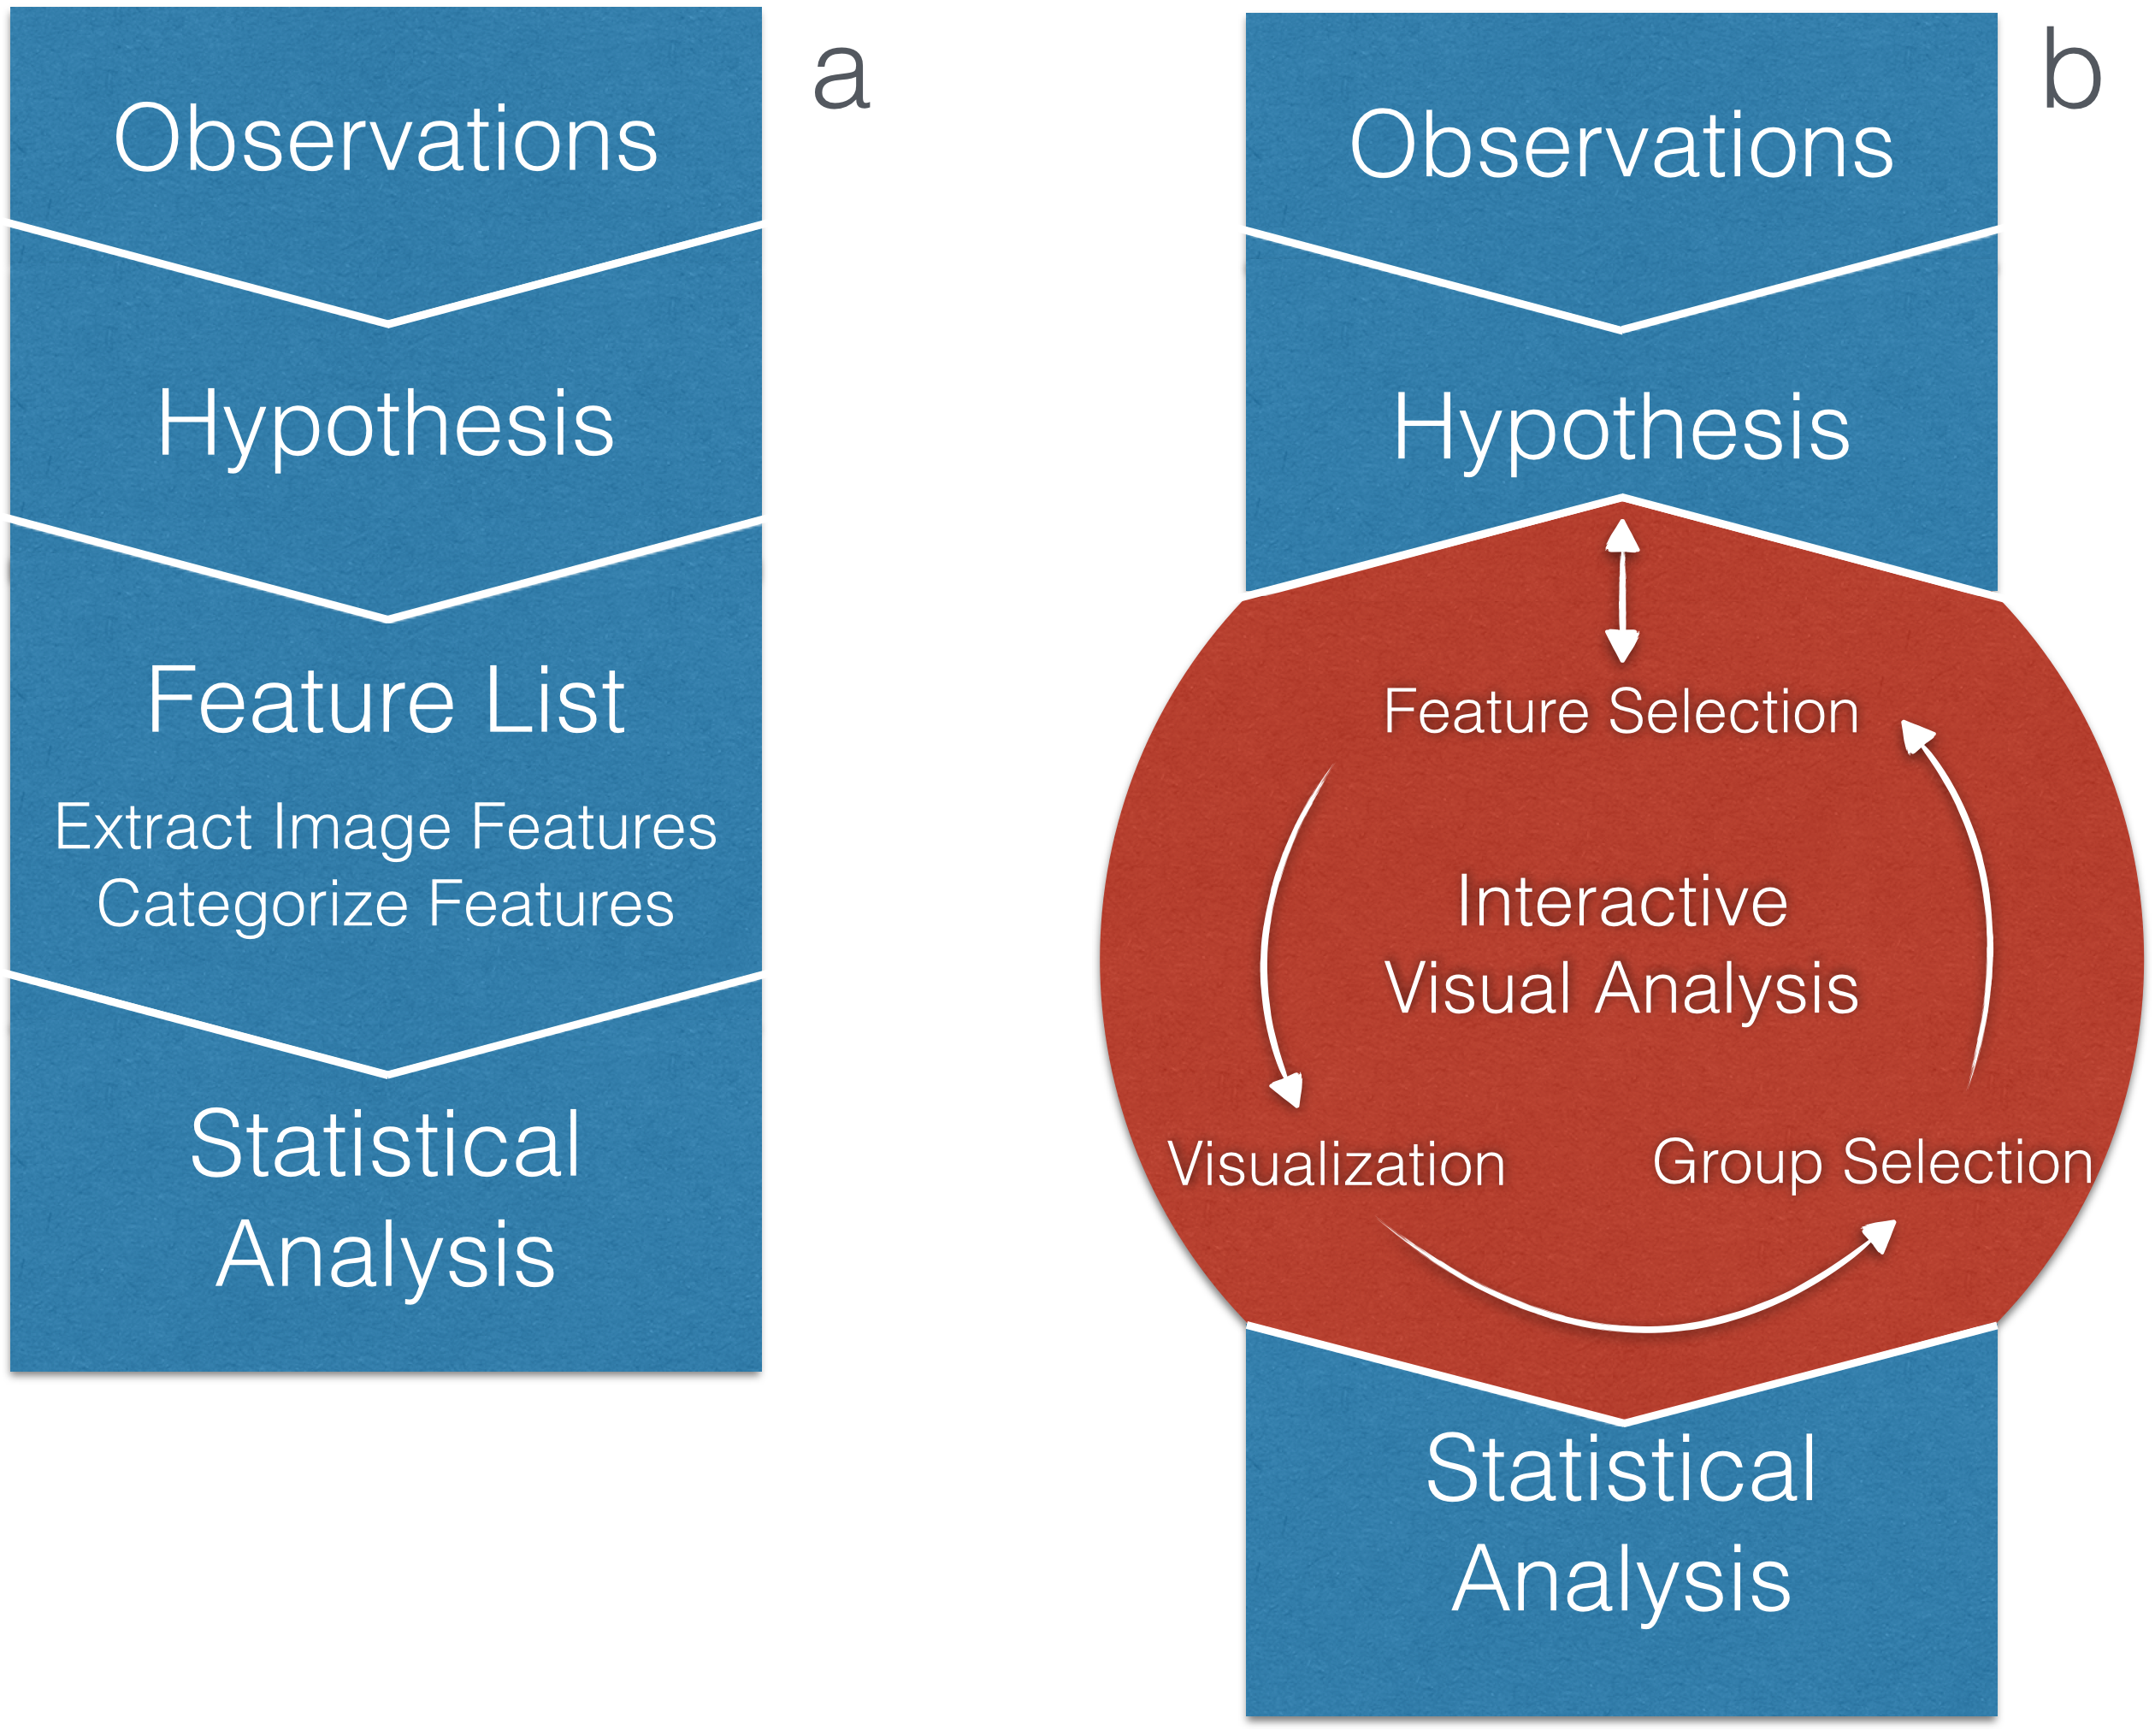
\includegraphics[width=3.0in]{figures/workflow_comparison}
 \caption{ToDo Abbildung noch nicht final. Visual Analytics systems are able to complement parts of the epidemiological workflow, not replace it. The appropriate combination of statistical- and interactive driven analysis shows promising potential to unveil the information in the data. (a) shows the standard epidemiological workflow, (b) the IVA supported one. The iterative red highlighted part is called the \emph{IVA Loop}.}
\end{figure}
%
As described in subsection~\ref{EpidemiologicalWorkflow}, the epidemiolgical workflow is a strict sequence of steps taken by domain experts and needs to be reproducible and comprise statistical integrity.
%
Figure~\ref{fig:WorkflowComparison} (a) describes this workflow as consecutive series of steps.
%
The workflow we propose by introducing the \emph{IVA} principle into the epidemiological application domain does not aim to replace the existing workflow but to complement its weaknesses.
%
In the current state the workflow treats the data like a black box.
%
A list of features describing the hypothesis is compiled and analyzed using statistical tests. 
%
The resulting value decides whether the data supports the hypothesis or not.
%
It would be possible that there actually are features of the data set which support the hypothesis by discriminating the population in the expected way, but with this approach they are not highlighted in any way.
%
This becomes even more imminent when the workflow is adapted to the analysis of the medical image data.
%
Domain experts annotate tediously landmarks which allow to derive metrics like distances which are then handled like other features and analyzed using the same set of statistical tools.
%
Not only does this leave out the majority of the information in the medical image data by abstracting it to single values, it is easily possible that information left out would heavily influence the result.
%
Considering more complex parts of the data would make those results more trustworthy and also could identify possible anatomical confounders--an epidemiolgical research result in itself.
%
Statistical tests check for validity of the number but not for their completeness or plausibility!
\\\\
\emph{IVA} tries to illuminate the black box by making the domain experts part of the feature list selection process.
%
Figure~\ref{fig:WorkflowComparison} (b) highlights the iterative process as part of the epidemiolgical workflow.
%
Note that it also aims to project back into the hypothesis formulation step to amplify hypothesis generation 
%
This has to be handled with care since overfitting of expectations to the available data is an imminent danger as described by Turkay and colleagues \cite{Turkay2013}.

\subsection{Image Centric Cohort Study Data in Interactive Visual Analytics Context}
In the \emph{IVA} context, data is divided into two major view types.
%
The human body exposing shape information for the \emph{physical view}, also referred as the \emph{independent variable} \cite{Oeltze2013}.
%
This information space is usually displayed via volume rendering techniques \cite{Oeltze2007}.
%
%Spatiotemporal views include data from the \emph{Object Space Domain} renders data centered to the focused domain, in our example the medical image data space.
%
\emph{Dependent variables} in the epidemiological context can be divided twofold:
\begin{itemize}
	\item Variables derived from the image data. 
	%
	These measures abstracts shape information as quantification to allow for comparison. 
	%
	These variables describe image data and can also be used to brush in the image space.
	\item Epidemiological socio-demographic or medical attribute data.
	%
	These values belong to every subject which is represented in the image space, but does not describe shape information.
	%
	This is the data epidemiologists usually want to correlate with image data.
\end{itemize}
%Other data associated to elements in the object space are considered to be the \emph{Attribute Space Domain} and are displayed using various range based views using statistical graphics and information visualization techniques like scatterplots, bar charts or parallel coordinates \cite{Oeltze2013, Oeltze2007}.
%
%Specific for the epidemiological application domain is that both Object- and Feature Space Domain influence the outcome of interest.
% \textbf{Object Space}\\
% - Medical Image Data / Spine Segmentations\\
% \textbf{Attribute Space}\\
% - SHIP-Variables\\
% - Derived visualizations
% 
% ? Where to incorporate Levels of IVA

\subsection{Data Preprocessing}
To include heterogenous epidemiological data in an \emph{IVA}-framework it is necessary to process it to obtain standardized views to the available features.
%
Due to the different acquisition modalities there have to be different techniques incorporated.
%
Data obtained using questionnaires or medical tests are often stored using statistical packages like \texttt{SPSS} or \texttt{Stata} which have a proprietary data format with limited export capabilities.
%
The best solution for us was to simply export the data in the respective tool to a character separated text file and then convert it to data types which are easier manageable like JSON or XML using our own classes.
%
In order to verify that the conversion worked as expected and the data is valid it is good practice to use data wrangling tools like \texttt{OpenRefine} to validate the data.
%
Exporting the data dictionary which stores information about each manifestation of a feature is also an important step to get a detailed description of data variables and the meaning and unit of measurement of their values.
%
Since the reasons for missing data have a wide range from ethical to medical and personal issues, these are also included as error codes which have to marked as such in the data dictionary.
\\\\
Processing the image data associated to each subject consists for the most part of information extraction about a structure of interest.
%
This is either done manually by experts setting land marks (sometimes supported by algorithms connecting the land marks like Graph-Cuts) or by a (semi)-automatic detection, registration and segmentation.
%
Algorithms applied to the data do not only have to deal with a large inter-subject variability of the structure of interest but also needs to be reproducible \cite{Preim2014}.
%
Model based approaches have shown to be effective for this task \cite{Gloger2010, Gloger2012, Rak2013}.
%
If a segmentation yields only binary masks separating the structures, algorithms like Growing and Adaptive Shapes can be applied creating a surface grid where each point is comparable throughout the population \cite{Ferrarini2007}.
%
Intensity based comparison can be achieved using rigid image registration, but model based results however are preferable \cite{Klemm2012}.
%
Comparison based on grey values is usually carried out to to measuring the quantity of fat, water, and--application specific--iron content (liver) or distribution of grey and white brain tissue.

Morphometric variables are derived to allow for statistical comparison of the tissue which incorporate mostly position, volume and relative distances and alignment to other structures.
% 
% - Data Format\\
% - Missing Data\\
% - Registration of Image Data (VMV'12)\\
% - Extraction of Image Parameter

\subsection{IVA Patterns}

The explorative procedures when analyzing data using \emph{IVA} can be divided into three different patterns, handling interaction between domain and range variables.

\subsubsection{Local Investigation}
This pattern projects information from image space to the range perspective.
%
As opposing to other \emph{IVA} application domains this step is more complicated in the epidemiological context.
%
Shape information can not be brushed by incorporating ROI-selections but rather has to employ techniques that specify local deformation changes \cite{Hermann2014} or subjects that belong to a shape class.
%
Methods available for \emph{feature selection} strongly depend on the type of registration that was applied to extract the tissue of interest.
%
Model based segmentations or masks yield data structures capable of calculating mean shapes and distances between individuals or subject groups.
%
Feature selection is also possible by applying clustering algorithms in order to get shape-groups \cite{Klemm2013VMV}.
%
These algorithms can be used to investigate interactions between shape-groups and other non-image based variables.
%
Another application is the outlier analysis.
%
Outliers can indicate segmentation errors or an outstanding group of individuals who may share a pathology.

% Local Investigation
% - Projection from Image Space to Attribute data. This is more difficult in our application, because we currently only brush on derived features.\\
% - Clustering in Image Space yields Groups which can be analyzed using the attribute space\\
% - Create a Pipeline Overview over different Levels of different IVA Patterns and Stages

% \subsection{Feature Selection}

% \subsection{Brushing the information space}
% - derive new groups which serve as input for the feature selection

\subsubsection{Feature Localization}
% Subset selection of range variables yields features
As described before, the vast majority of data points are considered to be dependent with respect to the image domain in the \emph{IVA} context.
%
Selecting subjects based on image derived data can be seen as additional possibility of shape-related grouping.
%
For the most part the epidemiologist is interested in the shape of subjects within a range of a set of variables that describe the current hypothesis.
%
Epidemiologists are used to categorize data into groups that fit their hypothesis formulation.
%
Continuous variables like age are for example often divided in categories like young, aged and elderly.
%
Categorization is strongly dependent on the hypothesis and therefore requires suitable brushing techniques as described in section~\ref{sec:AdaptiveFeatureVisualization}.
%
%To gain insight into interactions between SHIP-

% - Selection of Information using Bar Charts, Scatterplots or Parallel Coordinates which projects the selection into the Object space\\
% - this selection is for categorical data already given implicitly bei projecting the 3D-View onto the Bar Charts/Mosaik Plots!\\
% - this aims to locale features of the data!\\
% - Gain Information about SHIP-Variables by putting them into the context of each other. The Pivot Table allows for direct numerical\\ analysis, while the information visualizations allow for better insight of the combination

\subsubsection{Multivariate Analysis}
%Introduced in the information visualization, the multivariate analysis means selecting subjects in like in the feature localization step and get have the result highlighted in another linked view displaying other non-image parameter.
Introduced in the information visualization, the multivariate analysis incorporates brushing and linking of of views displaying non-image parameter.
%
%This represents for the most part the usual approach which essentially is the analysis of how variables interact with each other, only in a visual analysis context.
%
Special for the application domain is the need of statistic measures which describe how variables correlate with each other given the selected groups.
%
These association also summarized using Pivot Tables which are popular in epidemiology and which are described in the following section.
% - Selection of Elements in Scatterplots, Barcharts or Parallel Coordinates Views - observe how selection changes another view - this allows for multivariate analysis\\
% - Becker, R.A., Cleveland, W.S.: Brushing scatterplots. Technometrics 29(2) (1987)\\
% - Wang Baldonado, M.Q., Woodruff, A., Kuchinsky, A.: Guidelines for using multiple views in information visualization. In: AVI ’00: Proceedings of the working conference on Ad- vanced visual interfaces, pp. 110–119. ACM Press, New York, NY, USA (2000). DOI\\ http://doi.acm.org/10.1145/345513.345271
% - By brushing individual parameters or create new binnings of parameter it is possible to see how they change in coordinated views. This is already implemented in the Cargo framework\\
% - by creating comparative 3d Visualizations it is possible to assess the influence of non-image parameters to the visual space.

\section{Interaction- and Visualization Techniques}
%
We employ the fourth and highest level which includes next to brushing and linking, advanced brushing, extraction of attributes the development of visualizations custom tailored to the data sets.
\begin{figure}[htb]
 \centering
 %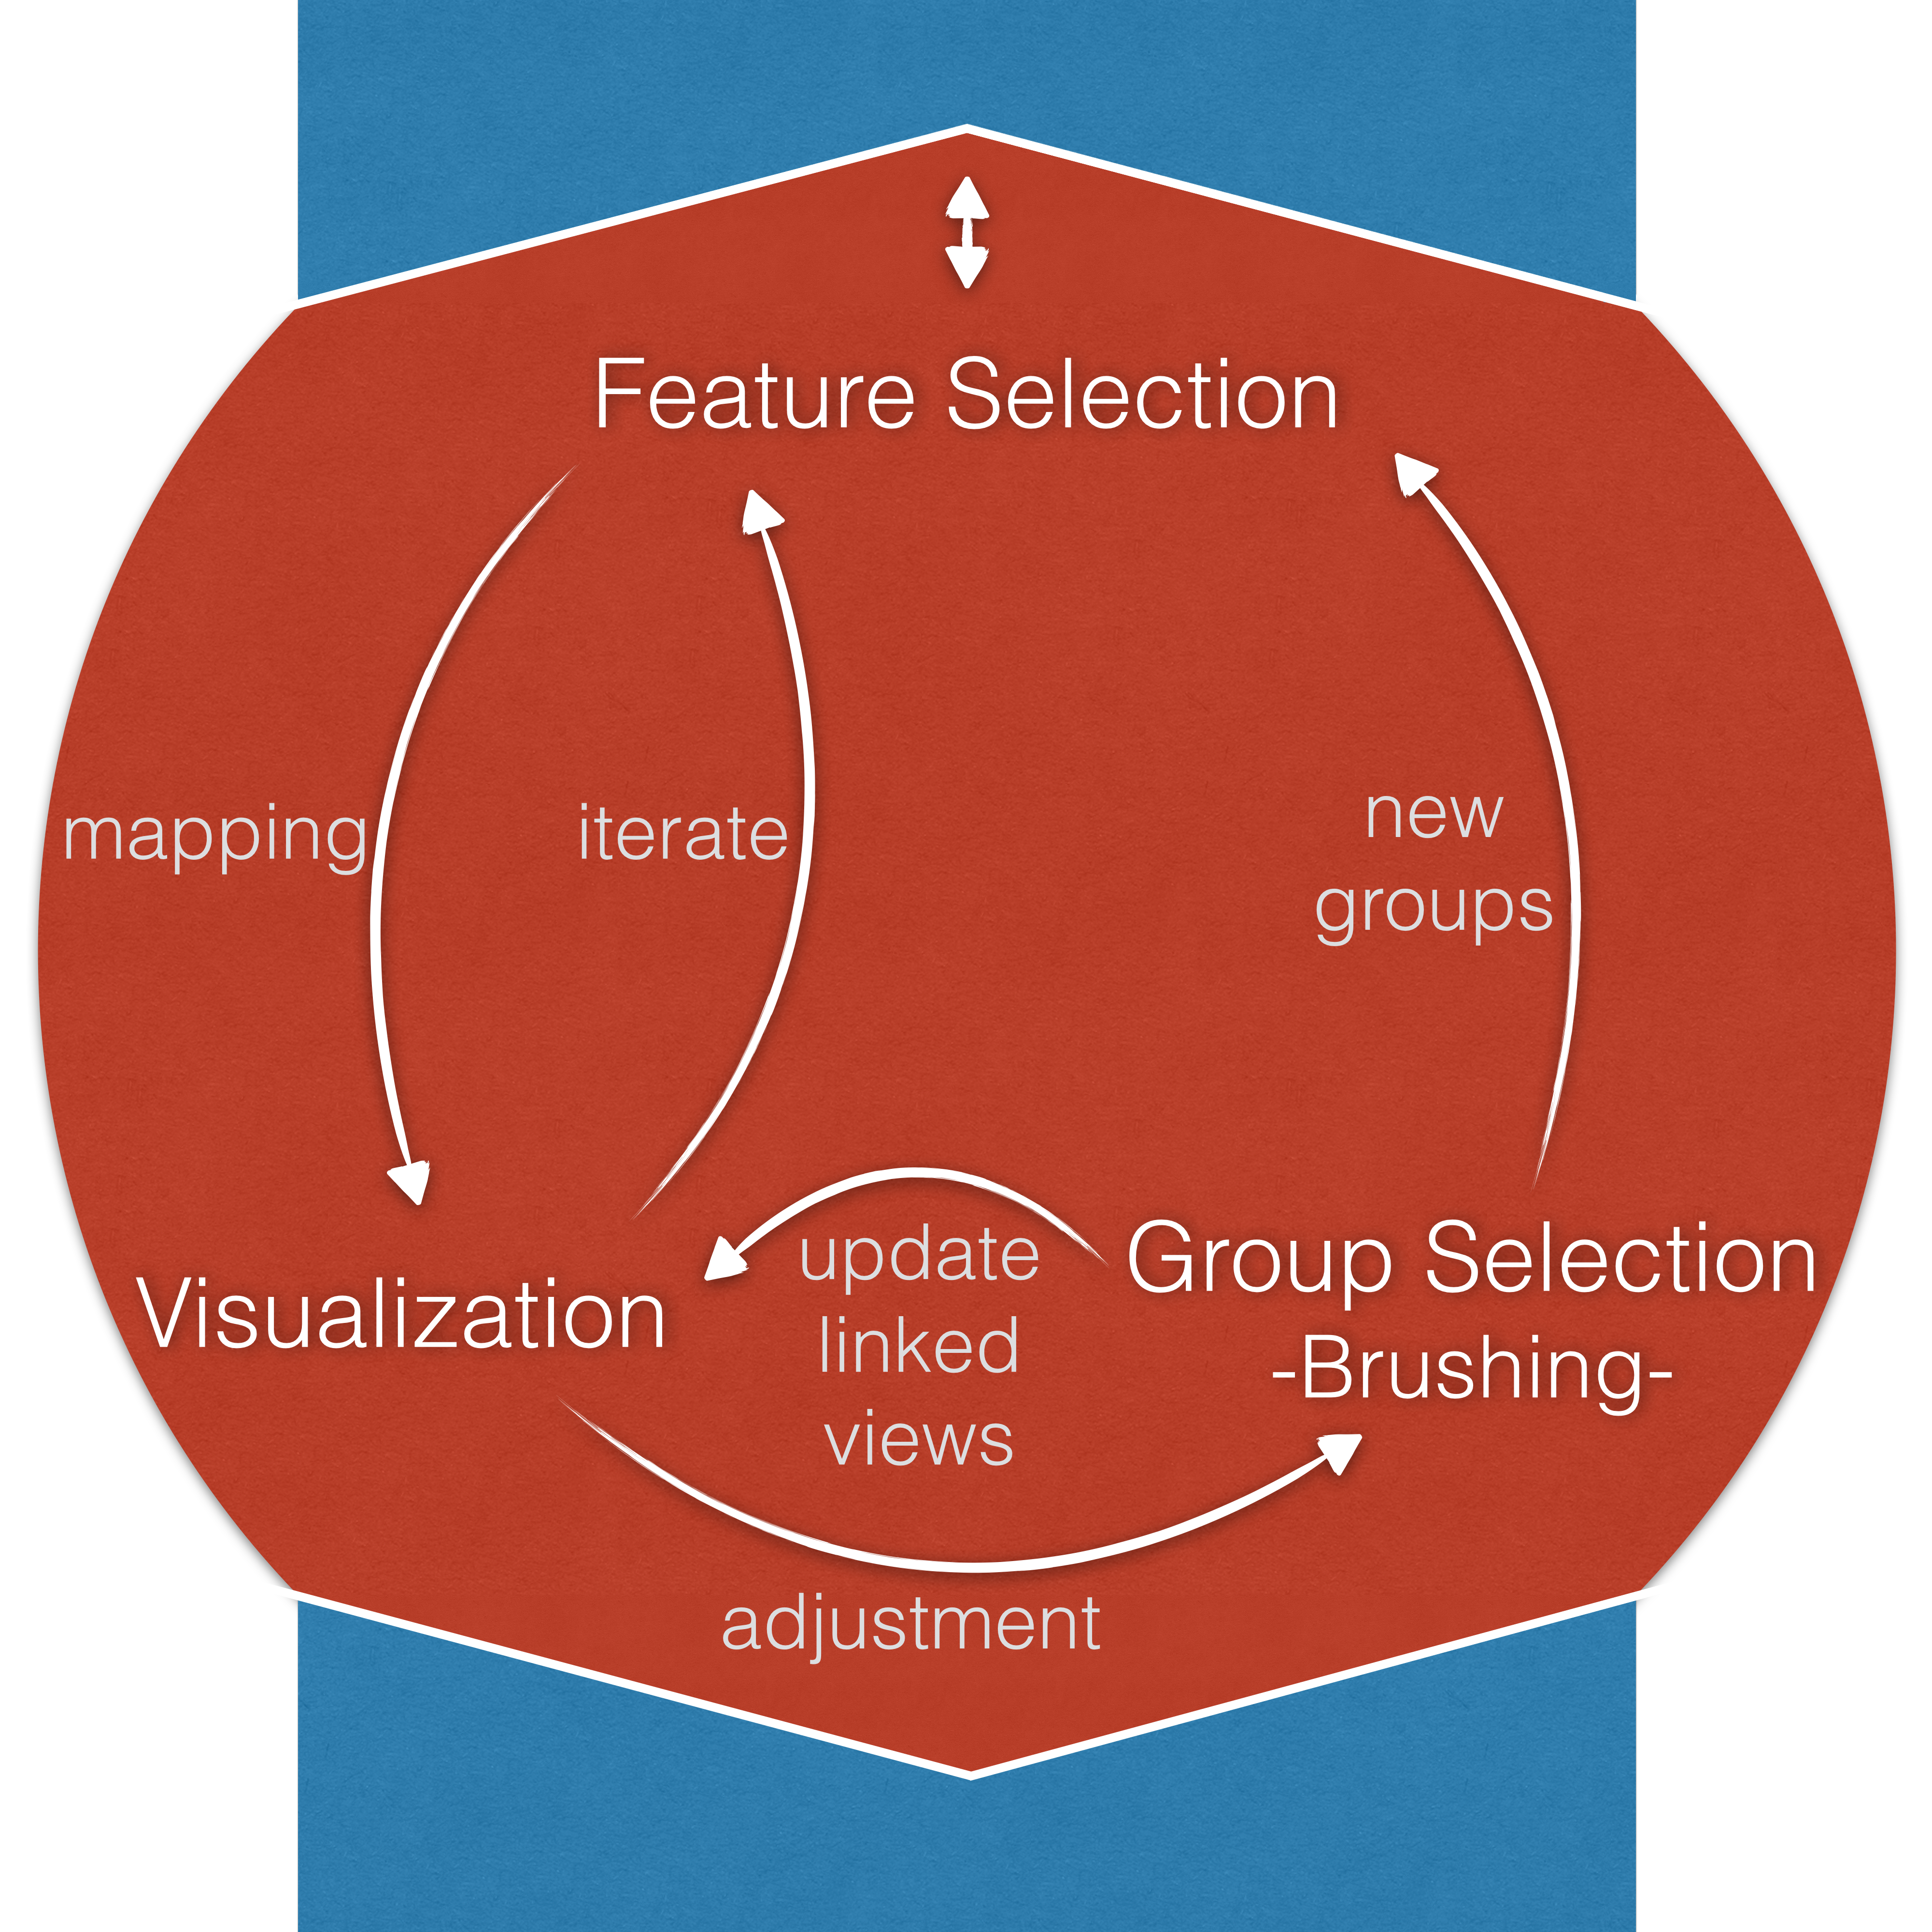
\includegraphics[width=1.5in]{figures/InteractionLoop}
 \includegraphics[width=3.5in]{figures/visualization}
 \caption{\emph{Image is not final} Screenshot from the front-end which is divided as follows: (a) Sidebar which contains all features as well as the groups defined in the analysis process; (b) Canvas area where features can be added via drag and drop and the visualization chosen automatically according to the data type; (c) Interactive Pivot Table which shows exact numbers for each displayed variable combination. The data displayed is used to analyze the lumbar spine.
 }
 \label{fig:visualization}
\end{figure}
\emph{IVA} levels define different levels interaction. 
%
The employed techniques needs to respect the epidemiological affordances.
%
Hypothesis generation bears the chance of over-fitting the data to expectations.
%
To avoid this, a timeline needs to be introduced which keeps track how many variable variations the user evaluated before coming to an conclusion.
%
Since epidemiologists are used to process groups based on table representations we decided to introduce an interactive solution in form of a Pivot Table.

\subsection{Structure and Workflow}
We divide the workspace into three major parts as seen in Figure~\ref{fig:visualization}.
%
\begin{figure}[htb]
 \centering
 \label{fig:InteractionLoop}
 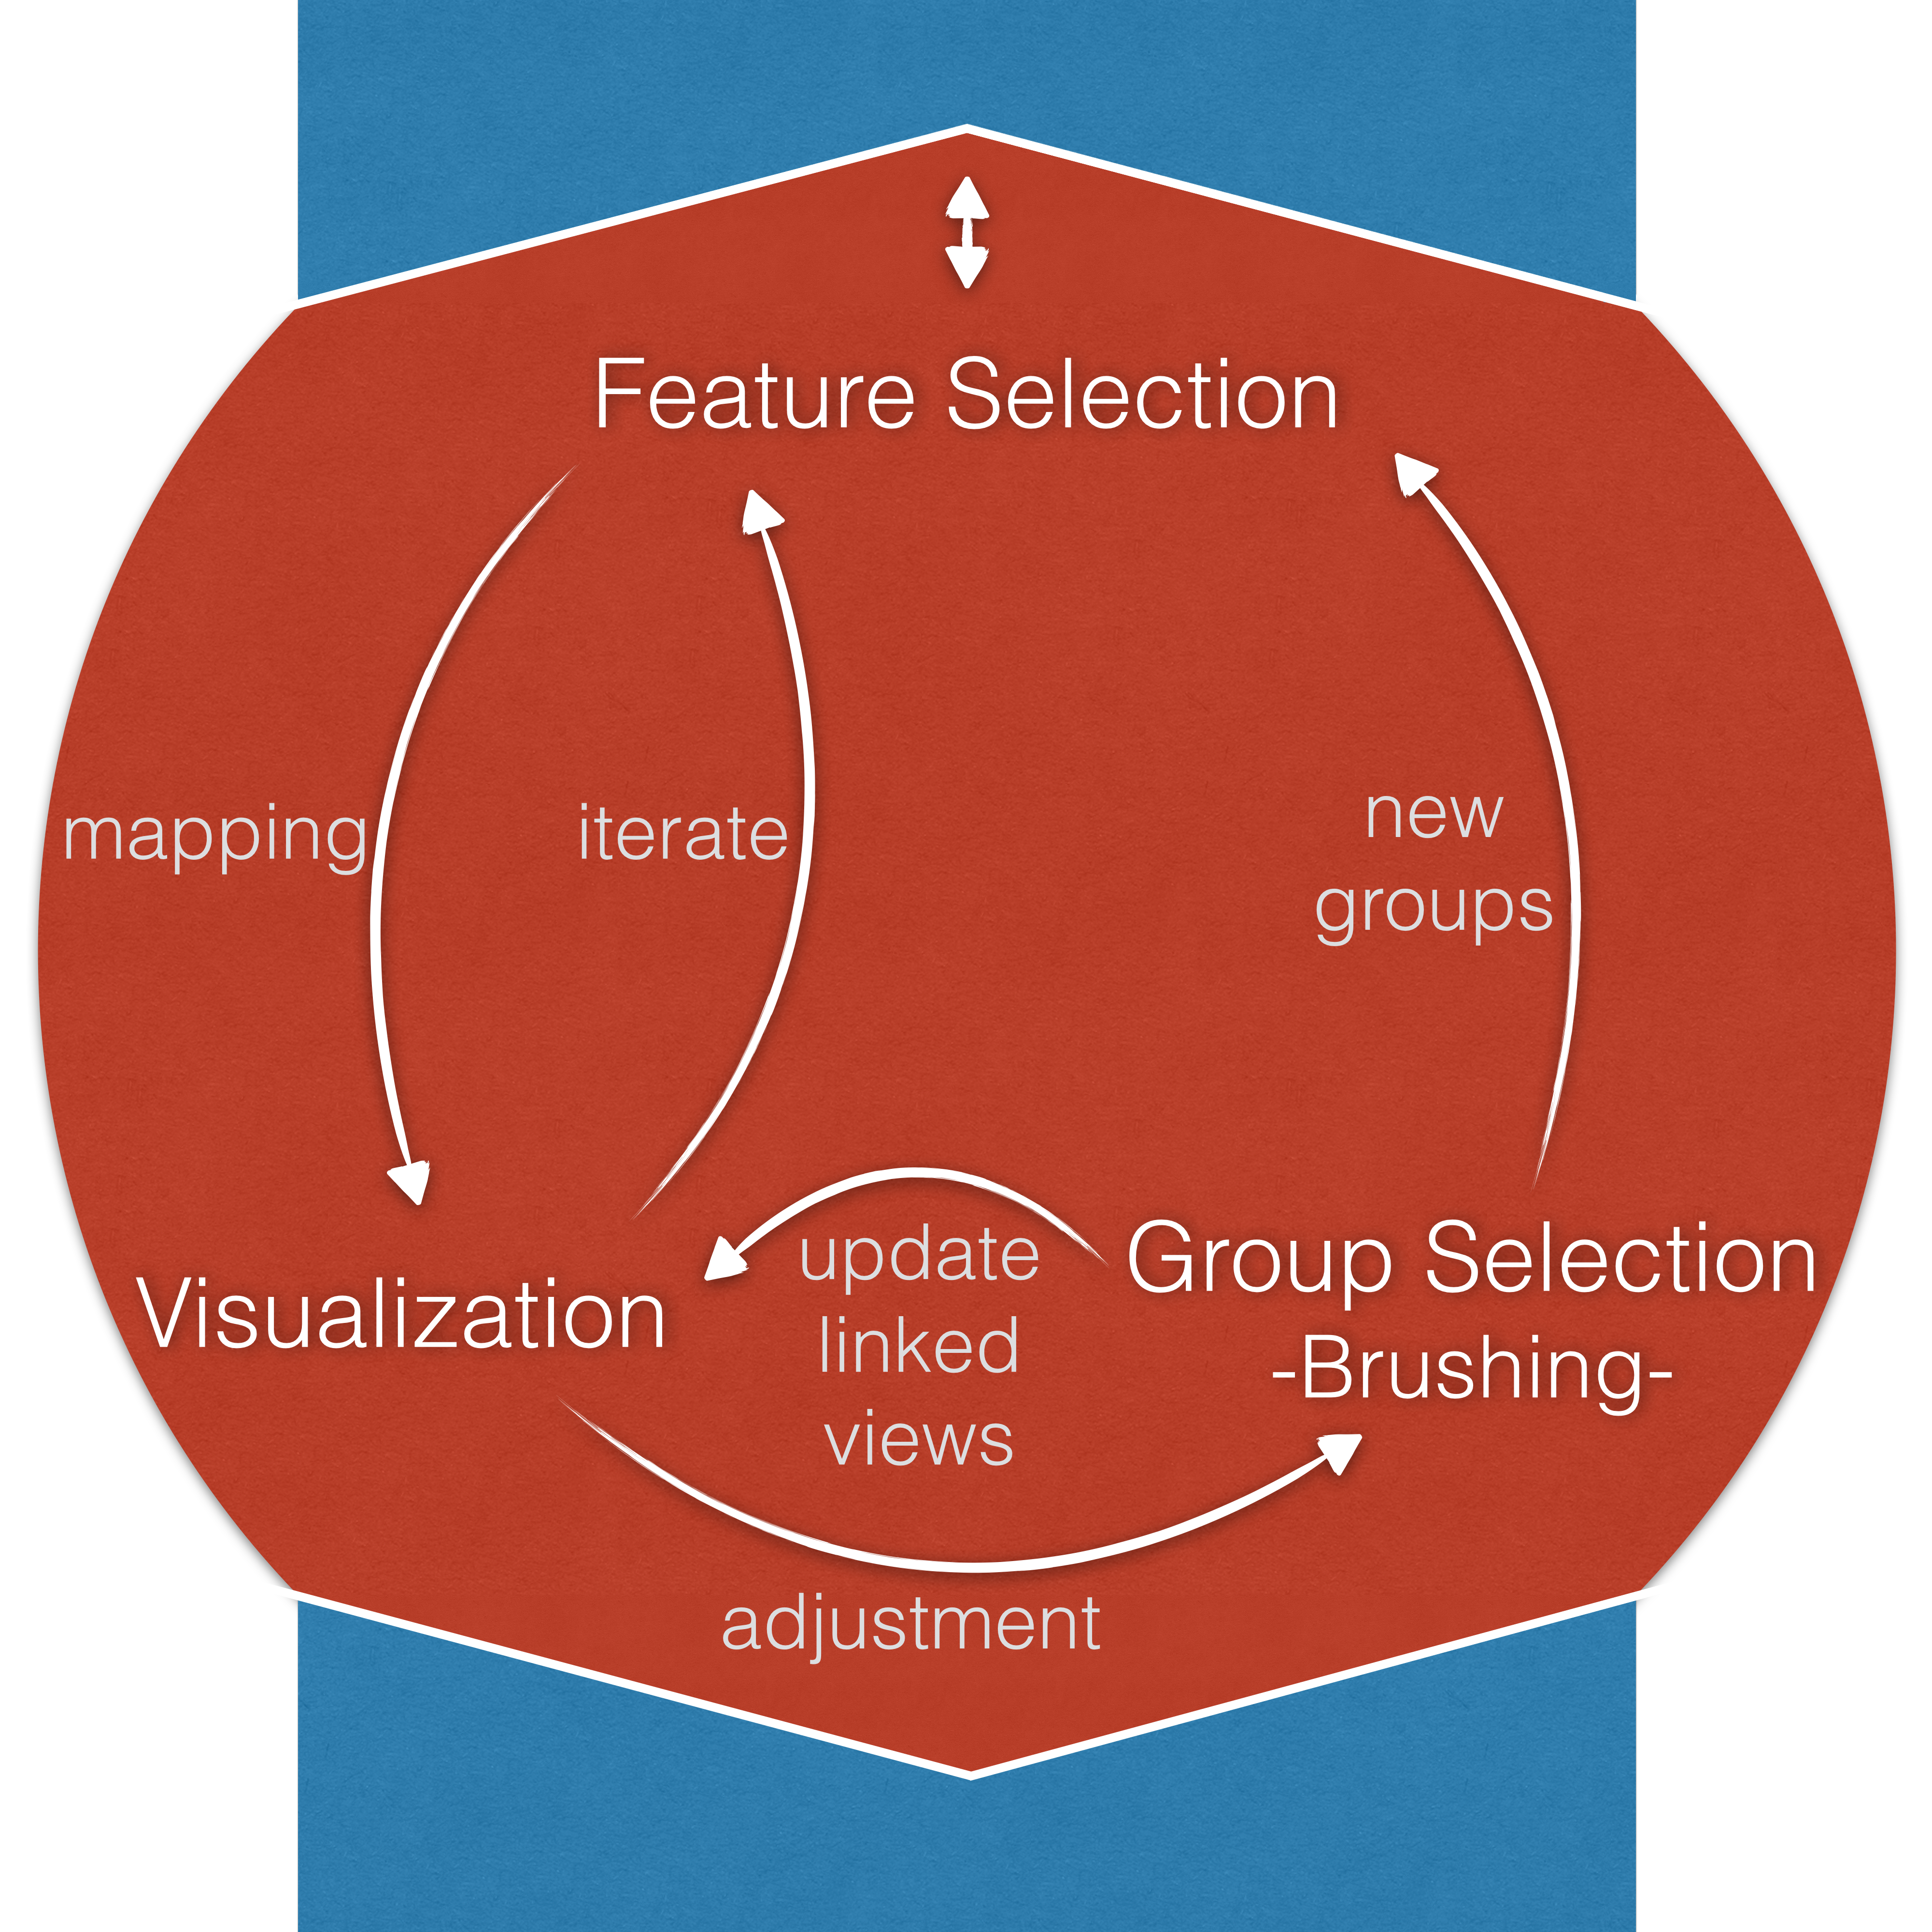
\includegraphics[width=3.0in]{figures/InteractionLoop}
 \caption{Detailed Version of the \emph{IVA Loop}. Usually starting with a selection of Variable of interest (user-driven or via data mining techniques), the data is mapped using a visualization technique appropriate for the selected data types. The data is visualized in the independent and dependent domain space, which can then be brushed, yielding new groups which can be investigated using further variables. Note that adjacent steps are directly connected via feedback loops allowing for iterative refinement and give as much freedom to the user as possible.}
\end{figure}
TODO auf Fig~\ref{fig:InteractionLoop} zurückkommen
%
The sidebar holds all available variables as well as groups either derived by user input or automatic clustering.

From the sidebar, elements of interest can be put into the canvas area via drag and drop.
%
Doing so will automatically create a information visualization suitable for the current data type.
%
3D shape information about the investigated structure is displayed for each variable manifestation.
%
By dropping variables on existing visualizations the system creates a visualization that allows for comparison (e.g. mosaic plots for ordinal variables).
%
Elements can be brushed in the information visualizations and are linked to the other representations in the canvas.
%
Shape based clustering can either be applied to all subjects or subgroups.

All elements in the canvas view are also represented in the interactive Pivot Table which gives detailed information how the subjects are distributed given the displayed variables.
%
Details to the different views are presented in the following sub-sections.

ToDo\\
- wie werden Confounder gefunden?\\
- welche statistischen Kennzahlen werden eingebunden?\\

\subsection{Sidebar}
A overview of all variables is presented in a sidebar where they are categorized to different types like somatometric, disease- or lifestyle related, pain indicators and laboratory data.
%
It also contains subject groups either defined by user brushing or by automated clustering.
%
Groups are treated exactly like other variables since they work exactly the same way which is dividing the subject space into different labeled categories.
% TODO Implement
Bar charts show the distribution of manifestations of each variable in the sidebar.

\subsection{Adaptive Feature Visualization} \label{sec:AdaptiveFeatureVisualization}
Inspired be the previously discussed \emph{GPloms} \cite{Francois2013} the visualization type is chosen dynamically based on the variable types and number of visualizations which need to be displayed.
% TODO Implement MOSAIC PLOTS, Scatterplots, Parallel Coordinates
If possible the medical image data is directly included into the plot as well by including mean shapes for each manifestation (Figure~\ref{fig:visualization} (b)).
%
The 3D-plots can be navigated using standard mouse inputs and the camera is synced so that a direct comparison is given.
%
If a feature is dropped on an existing plot, the visualization changes dynamically to properly make them comparable. 
%
Each plot can be brushed using widgets.
%
It is able to duplicate brushes in order to create new groups which are evenly spread out.
%
A use case for this is when a continuous feature has to be divided into even groups.
\\
ToDo\\
- Dichotomous data\\
- Time-Line\\
- Statistical Analysis (Odds ratios)

\subsection{Pivot Tables}
When opening a random epidemiological paper the reader will in almost all cases find some sort of pivot table to present the data.
%
As seen in Figure~\ref{fig:visualization} (c) it is a good way to display how many subjects are in each group.
%
Pivot table quickly get confusing and cluttered when they are divided into to many subgroups.
%
We tackled this problem by making the order and number of displayed variables adaptable.
%
This also applies on the designation of Row or Column Variables.
% TODO IMPLEMENT
The mean shape for each resulting sub-group is also displayed for each subject.

\subsection{Automated Feature Suggestion}
As discussed previously, highlighting potential interesting values in the data set is one major benefit of the \emph{IVA} powered approach.
%
Turkay and colleagues used the approach to calculate various key figures based in the distribution functions of each feature derived from the image data \cite{Turkay2013}.
%
Since the majority of our data are categorical features, we have to employ different solutions.
%
A solution for this problem are odds ratios, which are a standard statistical tool for stating relations between features.
%
Odds ratios can only be calculated for $2\times2$ contingency tables which usually represent the presence of a condition in a population divided by a characteristic (e.g. male/female subjects with presence or absence of back pain).
%
To calculate odds ratios for variables with more than two manifestations, we calculate local odds ratios for each possible combination, yielding a matrix for each feature combination \cite{Rudas1998}.
%
When the subjects are divided into groups and the calculation is carried out again for all feature combination, the difference in sum of the odds weighted with the number of manifestations per feature can be used to indicate if the feature combination yields a difference.
%
These difference are then highlighted in a separate tab of the side bar "Interactions".
%
Interesting interactions then can be assessed creating a linked view using the standard drag and drop workflow.
\\\\
In the following sections we will discuss details on the implementation which relies on modern Web-Technologies.
\\\\
ToDo\\
- This can be improved--summing up the values possibly not the cleverest solution--calculation of variance etc. possible\\
- Matrix Visualization?



\subsection{Implementation}
\begin{figure}[htb]
 \centering
 \label{fig:technologies}
 %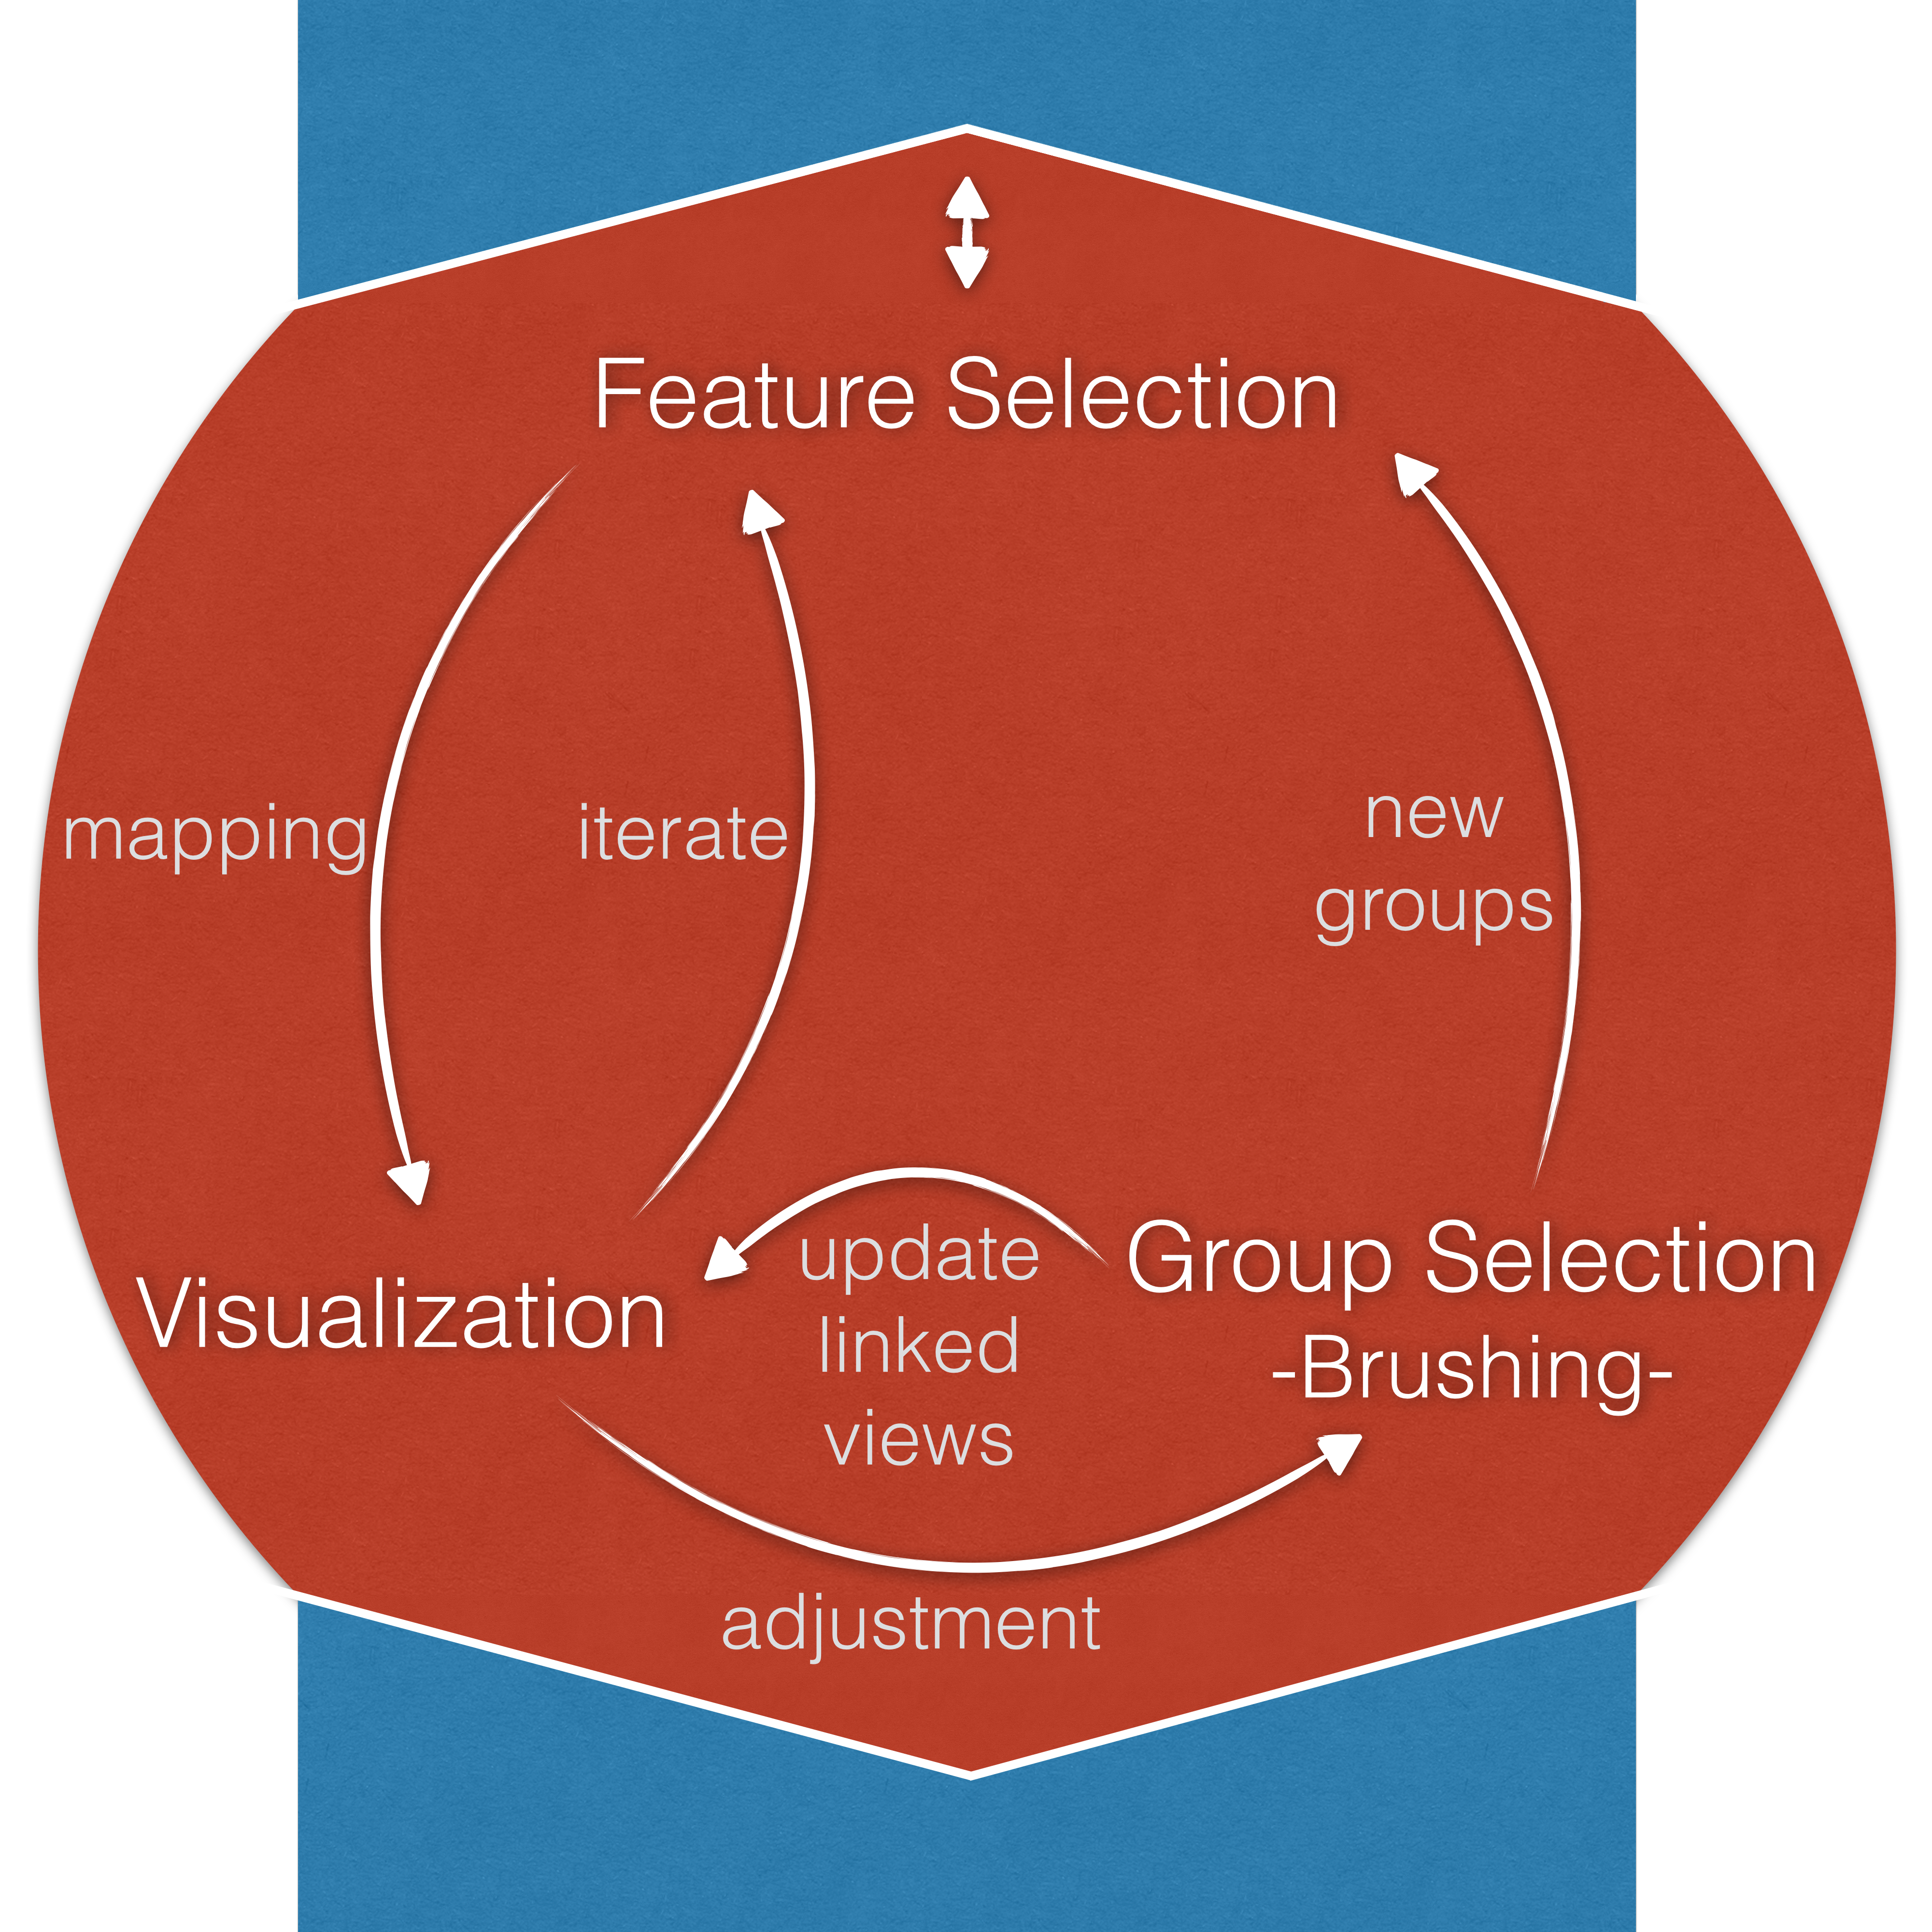
\includegraphics[width=1.5in]{figures/InteractionLoop}
 \includegraphics[width=3.5in]{figures/technologies}
 \caption{\emph{Image is not final}. The front-end solution (left) uses state of the art web technologies like HTML5/CSS3, WebGL and SVG to display the data.
 % 
 The NodeJS based back-end (right) stores all image- and non-image data and transfers it to connected clients.
 %
 All computation heavy operations like calculation of mean-shapes or -distances as well as statistical processing is done by the server to keep hardware requirements of client systems low. 
 %
 Client-Server communication is accomplished via the WebSocket protocol.
 }
\end{figure}
%
In order to provide a fast communication loop between method development and expert input we decided to base all implementations on modern web technologies which benefits from various advantages:
\begin{itemize}
	\item No additional software needs to be installed, most people use decent state of the art web browser. If developed using proper standards, the applications even run on mobile devices. 
	\item The Client-Server structure allows it to employ heavy computation on a server machine and transfer results to the client
	\item Since Image data for several thousand subjects claims hundreds of Gigabytes disk space it can remain safely on the server and elements can be transferred on demand.
	%
	High confidentiality standards of the data can be met by restricting access via a account system
	\item Recent developments in WebGL applications running in browsers with near native performance push the development into to the web which results in many open source libraries which are well documented, rich in examples and driven by active communities.
\end{itemize}
These advantages do not come without drawbacks.
%
Many methods which specialized libraries like the Visualization Toolkit (VTK) or R for statistics have build in need to be written from scratch in order to fit in the context.
%

The back-end is written using Node, which based on the Google V8 Javascript runtime environment.
%
Due to its event-driven non-blocking I/O model it is fast and does not freeze in case of heavy workload like mesh calculation.
\\\\
Non-image data for all Subjects including the data dictionary is stored on the Server in a JSON file.
%
Image data is available as raw DICOM files as well as segmented Meshes which can be used to compare subjects.
%
On client connection the requested files are transferred.
%
The server processes calculation heavy statistical tasks like calculation of Odds Ratios or Chi Square tests for all variable combinations in order to keep the computation time on the client as low as possible.
%

The front-end is created using Twitter Bootstrap as foundation for the layout and basic UI elements using HTML5, CSS3 and Javascript.
%
Information Visualizations like Scatterplots and bar charts are created using the popular Data Driven Documents library which works well for attaching data to visible elements like vector graphics.
%
WebGL rendering is done using the Threejs which allows GPU Accelerated data rendering.
%
Communication between Client and Server runs through the WebSockets protocol.
%
Since our clustering algorithms are written in MatLab we hat to access them using the Node Server.
%
We accomplished this by converting them to parameterized standalone console applications which are spawned by node on client request and then reads the result from the console standard-out and returns it in a proper format to the client.
%
All parameter steered console applications can be incorporated in this context.

\section{Application}
\subsection{The Spine Dataset}
- Describe steps from gathering Information from the raw image files (segmentation, abstraction, visualization)\\
- Problem of sparse differences - Visualization has to be more abstract to emphasize the differences.\\
- Input of Epidemiologists goes here!\\
\\\\
\textbf{From VMV'13 Paper}\\

All whole-body MRI scans were acquired on a 1.5~Tesla scanner (Magnetom Avanto; Siemens Medical Solutions, Erlangen, Germany) by four trained technicians in a standardized way. Subjects were placed in the supine position. Five phased-array surface coils were placed to the head, neck, abdomen, pelvis, and lower extremities for whole-body imaging. The spine coil is embedded in the patient table. The spine protocol consisted of a sagittal T1-weighted turbo-spin-echo sequence (676 / 12 [repetition time msec / echo time msec]; 150$^\circ$ flip angle; 500~mm field of view; $1.1\times1.1\times4.0~mm$ voxels) and a sagittal T2-weighted turbo-spin-echo sequence (3760 / 106 [repetition time msec / echo time msec]; 180$^\circ$ flip angle; 500~mm field of view; $1.1\times1.1\times4.0~mm$ voxels). First, both sequences were placed over the cervical and upper thoracic spine. Then, they were placed over the lower thoracic and lumbar spine. The MRI software automatically composed a whole spine sequence from the two T1-weighted and T2-weighted sequences \cite{Hegenscheid2013}. We were provided with 490 data sets.

%The model is placed in the scene using an empirically chosen initialization point. The force acting on the model stems from aggregation of loads, which are derived from a potential field resulting from a weighted sum of the T1- and T2-weighted MRI images, see \cite{Rak2013}. After detecting all spines, we register the models because in a later clustering step we only want to capture the local deformation of the lumbar spine, not different locations in world space. The models are registered using the Kabsch Algorithm \cite{Kabsch1976}, which is designed to minimize the root mean squared deviation between paired sets of points.
The model is placed in the scene using an empirically chosen initialization point. The force acting on the model stems from aggregation of loads, which are derived from a potential field resulting from a weighted sum of the T1- and T2-weighted MRI images, see \cite{Rak2013}. After detecting all spines, we register the models because in a later clustering step we only want to capture the local deformation of the lumbar spine, not different locations in world space. The models are registered using the Kabsch Algorithm, which is designed to minimize the root mean squared deviation between paired sets of points.
The model-based detection captures information about the spine canal curvature as well as the alignment of the vertebrae. It is not meant to capture information about vertebrae deformation and differences in spine canal extent.

\section{Summary and Conclusion}

%% if specified like this the section will be committed in review mode
%\acknowledgments{SHIP is part of the Community Medicine Research net of the University of Greifswald, Germany, which is funded by the Federal Ministry of Education and Research (grant no. 03ZIK012), the Ministry of Cultural Affairs as well as the Social Ministry of the Federal State of Mecklenburg-West Pomerania. Whole-body MR imaging was supported by a joint grant from Siemens Healthcare, Erlangen, Germany and the Federal State of Mecklenburg-Vorpommern. The University of Greifswald is a member of the ‘Centre of Knowledge Interchange’ program of the Siemens AG. This work was supported by the DFG Priority Program 1335: Scalable Visual Analytics.}

\bibliographystyle{abbrv}
%%use following if all content of bibtex file should be shown
%\nocite{*}
\bibliography{bibliography}
\end{document}
